In this section we discuss the characteristics of our infrastructure
and we clearly formulate the problem under analysis.

\begin{figure}[t]
  \centering 
  \usetikzlibrary{arrows}
\usetikzlibrary{automata}
\usetikzlibrary{positioning}
\usetikzlibrary{backgrounds}
\usetikzlibrary{fit}

\tikzset{
    state/.style={
           rectangle,
           rounded corners,
           draw=black, very thick,
           minimum height=0.6cm,
           minimum width=1cm,
           inner sep=3pt,
           text centered,
           node distance=0.9cm,
           },
    process/.style={
           rectangle,
           rounded corners,
           draw=black, very thick,
           minimum height=0.6cm,
           minimum width=1cm,
           inner sep=3pt,
           text centered,
           %node distance=1cm,
           },
    newprocess/.style={
           rectangle,
           rounded corners,
           draw=black, very thick,
           fill=lightgray,
           minimum height=0.6cm,
           minimum width=1cm,
           inner sep=3pt,
           text centered,
           %node distance=1cm,
           },
    processplaceholder/.style={
           minimum height=0.6cm,
           minimum width=1cm,
           %inner sep=3pt,
           text centered,
           %node distance=1cm,
           },
    closerstate/.style={
           rectangle,
           rounded corners,
           draw=black, very thick,
           minimum height=0.5cm,
           minimum width=5.32cm,
           inner sep=3pt,
           text centered,
           node distance=1cm,
           },
    abovish/.style={
           rectangle,
           rounded corners,
           draw=none,
           minimum width=1cm,
           text centered,
           node distance=1cm,
           },
    supercloserstate/.style={
           rectangle,
           draw=none,
           minimum height=0.2cm,
           minimum width=6.9cm,
           node distance=1cm,
           },
}

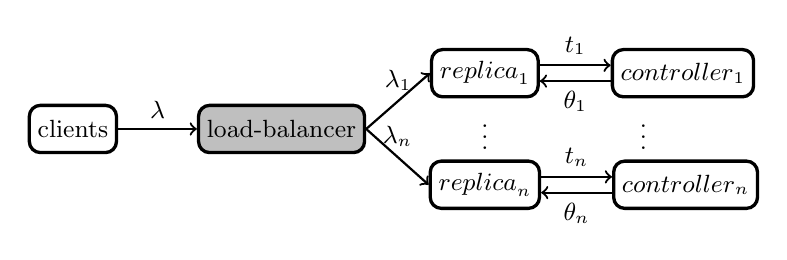
\begin{tikzpicture}[font=\small]
  \tikzstyle{surround} = [fill=black!20,very thick,draw=black,rounded
  corners, inner sep=5pt,] \tikzstyle{surroundblue} =
  [fill=blue!20,very thick,draw=black,rounded corners, inner sep=5pt,]
  \tikzstyle{surroundyellow} = [fill=yellow!20,very
  thick,draw=black,rounded corners, inner sep=5pt,]
  \tikzstyle{external} = [fill=none,very thick,draw=black,rounded
  corners, inner sep=15pt,]

% clients
\node[process] (clients){clients};

% load-balancer
\node[newprocess, right=1cm of clients] (lb){load-balancer};

% servers
\node[processplaceholder, right=1cm of lb] (replicaI) {$\vdots$};
\node[process, above=0cm of replicaI] (replica1) {$\text{replica}_1$};
\node[process, below=0cm of replicaI] (replicaN) {$\text{replica}_n$};

% controllers
\node[processplaceholder, right=1cm of replicaI] (controllerI) {$\vdots$};
\node[process, right=0.9cm of replica1] (controller1) {$\text{controller}_1$};
\node[process, right=0.9cm of replicaN] (controllerN) {$\text{controller}_n$};

% clients to lb
\draw[thick,->] (clients.east) -- (lb.west) node[midway, above] {$\lambda$};

% lb to replicas
\draw[thick,->] (lb.east) -- (replica1.west) node[midway, above] {$\lambda_1$};
\draw[thick,->] (lb.east) -- (replicaN.west) node[midway, above] {$\lambda_n$};

% replica to controllers
\draw[thick,->] ([yshift=+1mm]replica1.east) -- ([yshift=+1mm]controller1.west) node[midway, above] {$t_1$};
\draw[thick,<-] ([yshift=-1mm]replica1.east) -- ([yshift=-1mm]controller1.west) node[midway, below] {$\theta_1$};
\draw[thick,->] ([yshift=+1mm]replicaN.east) -- ([yshift=+1mm]controllerN.west) node[midway, above] {$t_n$};
\draw[thick,<-] ([yshift=-1mm]replicaN.east) -- ([yshift=-1mm]controllerN.west) node[midway, below] {$\theta_n$};

\end{tikzpicture}
 
  \caption{Architecture of a brownout-compliant cloud application
    featuring multiple replicas.}
  \label{fig:architecture}
\end{figure}

% CK: In cloud vocabulary, infrastructure generally refers to the physical hardware.
% CK: Hence, I prefer using "architecture" for "organization of software components".
Figure~\ref{fig:architecture} illustrates the software
architecture that is deployed to execute a brownout-compliant
application composed by multiple replicas. Our architecture
is widely accepted
as the reference one for cloud applications~\citep{Barroso09}. The
clients generate traffic to the cloud application, which is
balanced by a load-balancer and directed towards replicas. Each
replica implements the application logic. Special to our case is the
presence of a controller within each replica. The replica controller
takes care of adjusting the percentage of requests served with the
optional components enabled based on the measured response time of the
requests served by the replica.

More formally, we assume that clients generate requests for the
brownout application at a constant rate $\lambda$. These requests are
initially routed to the load-balancer. The load-balancer forwards them
to one of the $n$ replicas of the application. As a results, each
replica $i \in [1,n]$ receives requests at a rate $\lambda_i = w_i
\cdot \lambda$, such that $\sum_{i} w_i = 1$. $w_i$ are called the replica weights
and are dynamically computed by the load-balancer
according to its
load-balancing policy.

A replica $i$ responds to requests either partially, where only
mandatory content is included in the reply, or fully, where both
mandatory and optional content is included. The service rate for a
partial response is $\mu_i$ while a full response is generated with a
rate $M_i$. Obviously, partial replies are faster to compute than
full ones, since the optional content does not need to be prepared,
hence, $\mu_i \geq M_i$. Whether the replica serves requests partially
or fully depends on a parameter $\theta_i \in [0, 1]$, which
represents the probability of serving optional content. This parameter
is chosen by the replica itself, more precisely, by its controller. Assuming the replica is not
saturated, it serves requests fully at a rate $\lambda_i \cdot
\theta_i$ and partially at a rate $\lambda_i \cdot (1-\theta_i)$. To
aid load-balancing decisions, each replica piggy-bags the current
value of $\theta_i$ through the reply, so that this value can be
observed by the load-balancer.

The parameters $\theta_i$ are computed by controllers based on a
target average response time $\bar{\tau}$. Each replica $i$
periodically reports the average observed response-time $\tau_i$ to
its controller. In exchange, the controller adjusts $\theta_i$ to
maintain the average response-time close to its target value.

Within this architecture, we want to solve the problem of designing a
{\bf load-balancer policy}. Knowing the values of $\tau_i$ and $\theta_i$ for
each replica $i \in [1, n]$ and the arrival rate $\lambda$, our
load-balancer should compute the values of the weights $w_i$ such that
\begin{equation}
\sum_{i} \lambda w_i \theta_i
\end{equation}
is maximized. In other words, the load-balancer should maximize the
amount of requests served with the optional part enabled. In practice, this would also maximize
the application owner's revenue.
